\documentclass[sigconf]{acmart}
\usepackage{algorithm} 
\usepackage{algpseudocode}

 
\algdef{SE}% flags used internally to indicate we're defining a new block statement
[STRUCT]% new block type, not to be confused with loops or if-statements
{Class}% "\Struct{name}" will indicate the start of the struct declaration
{EndClass}% "\EndStruct" ends the block indent
[1]% There is one argument, which is the name of the data structure
{\textbf{struct} \textsc{#1}}% typesetting of the start of a struct
{\textbf{end struct}}% typesetting the end of the struct


\begin{document}


\title{On building a transfer graph for the evolution of pages in Wikipedia}



\author{César Di Meglio, 2042789}
\affiliation{%
  \institution{Utrecht University}}
\email{c.t.dimeglio@students.uu.nl}




\maketitle

\section{Introduction}
The velocity aspect of Big data leads to evolution and change over time in the information considered. Keeping track of those changes contributes into a better understanding of how data behaves with respect context throughout time. In this project, we measure the similarity of pairs of Wikipedia pages. If we consider one Wikipedia page, measuring its similarity to other pages can be an indicator of a trend. For instance, if we consider the page "Big data", modifications are made to it over time. These modifications will increase or decrease its similarity to other pages. At one time step, "Big data" could be more similar to "Apache Spark" than "SQL". This would mean that "Apache Spark" plays a larger role in "Big data" than "SQL" at the given timestep. The main challenge is to match the timesteps of our data. That is to say, we need to compare pages that have existed together at the same point in time. Aggregating these comparisons may serve as a representative estimate of how two pages relate to one another given a time frame (section \ref{sim entities}).\\*
How can we measure the temporal similarity of pages in time ?
The latter will be problematized in section \ref{problem}, solutions will be presented in section \ref{solutions}.
\section{Problem Statement}
\label{problem}
\subsection{Wikipedia pages as entities}
We denote $W$ as a set of Wikipedia pages, referred to as "entities". Each entity $w \in W$ is updated over time by Wikipedia users, we call each of those updates \emph{versions}. 
For each entity, we only consider the \emph{references} to other Wikipedia pages with respect to its versions. For instance, the entity "Utrecht" will have hyperlinks pointing to other pages like "The Netherlands" or "Amsterdam" given one of its versions.\\
Some pages are more or less regularly updated, we denote $\mathcal{N}(w) \in \mathbb{N}^*$ as the total number of versions since the creation of entity $w$ on Wikipedia. More formally, we have the following:\\
Let $w_i$ be a version of $w$ at a timestep $i$.
\begin{equation}
    \label{references}
    \forall w \in W ,\; \forall i \in \{1,..\mathcal{N}(w)\}, \; w_i = \{r_1,r_2,..\}
\end{equation}
where $r_j$ are the \emph{references} (to other Wikipedia pages) present in $w_i$.
The release \emph{date} of version $w_i$ is noted $\tau(w_i)$.
There are no versions of $w$ that where released at the exact same date (Eq.\ref{chrono}), these chronologically ordered (Eq.\ref{ordered}).
\begin{equation}
    \label{chrono}
    \forall (i,j) \in \{1,..\mathcal{N}(w)\}^{2} \;| \; \tau(w_{i}) \neq \tau(w_{j})
\end{equation}
\begin{equation}
    \label{ordered}
    \tau(w_1) < \tau(w_2) < ... < \tau(w_{\mathcal{N}(w)})
\end{equation}
where the relation "$<$" here means that the version on the left was released prior to the version on the right. The version $w_{\mathcal{N}(w)}$ is the latest one, that is to say, the one being displayed when searching $w$ on Wikipedia. 
From one version to another, \emph{references} can either be added, removed or kept the same.\
Let $w_i$ and $w_j$ be two versions of $w$ such that $\tau(w_i)<\tau(w_j)$, $(i,j) \in  \{1,..\mathcal{N}(w)\}$\\*
Either one of these three cases can happen:
\begin{equation}
    \begin{cases}
    \label{scenarios}
    w_i = w_j & \text{no new references were added from $i$ to $j$} \\
    w_i \subseteq w_j & \text{new references were added from $i$ to $j$} \\
    w_i \not\subseteq w_j & \text{references were deleted from $i$ to $j$}
    \end{cases}
\end{equation}
Note that in the third case of (\ref{scenarios}): $w_i \not\subseteq w_j$, new references could also have been added into version $w_j$.
\subsection{Measuring the similarity of entities}
\subsubsection{Definition: Measuring similarity}:\\
\label{blackbox sim}
We denote $ \mu : W \times W \rightarrow [0,1]$ a function that computes the similarity of two Wikipedia distinct \footnote{We neglect cases were $w$=$w'$ as property (\ref{prop}) always holds} pages $w$ and $w'$. Let $\epsilon \in ]0,1[$ be the \emph{similarity threshold}. We define the following property:
\begin{equation}
    \label{prop}
    (w,w') \in W^{2}, \,\mu (w,w') \geq \epsilon \iff w \text{ and } w' \text{are similar}
\end{equation}

\subsubsection{Similarity metric for two versions}:\\
\label{sim versions}
The similarity metric chosen to compare two versions of two Wikipedia pages is the \emph{Jaccard similarity}:
\begin{equation}
    \label{compare versions}
    \mu (w_i,w'_{j}) = \frac{\sharp(w_i\cap w'_{j})}{\sharp(w_i\cup w'_{j})}
\end{equation}
It consists of the ratio of the cardinalities of the intersection and the union of $w_i$ and $w'_{j}$. The latter measures the similarity in between the sets $w_j$ and $w'_{j}$ which contain references to other Wikipedia pages. This is a commonly used metric for measuring set similarity. It is also \emph{commutative} i.e: $\mu (w_i,w'_{i}) = \mu (w'_{i},w_i)$. If we had chosen a metric without this property, then we would have needed to make twice as much comparisons. Moreover, it fulfills the properties of the function evoked to in section \ref{blackbox sim}.
\subsubsection{Similarity metric for two entities}:\\
\label{sim entities}
In the scope of this project, we want to compare two Wikipedia pages given their respective histories. For the latter, the versions of the entities are computed using the metric defined in \ref{sim versions}. We say that a version of an entity is \emph{displayed}, if it is the one that appears when the entity is searched on Wikipedia at a given point in time.
The challenge is that we must compare versions of entities that were \emph{displayed} at the same time. 
\begin{figure}[H]
    \centering
    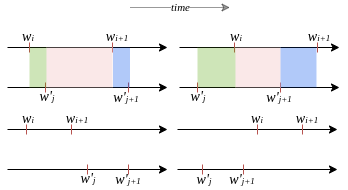
\includegraphics[width=200pt]{template/TimeDiff.png}
    \vspace*{-4mm}
    \caption{Overlapping configurations for $w_i$ and $w_j'$}
    \label{Overlap}
\end{figure}
Let $w$ and $w'$ be two entities we want to compare given their respective histories (see Fig. \ref{Overlap}). A version $w_i$ is \emph{displayed} from $\tau(w_i)$ included to $\tau(w_{i+1})$ excluded, $i \in \{1,...,\mathcal{N}(w)-1\}$.
In Fig.\ref{Overlap}, the two examples at the top (with the colors) exhibit configurations where versions can be compared because they are \emph{displayed} together at a point in time. Hence, for these examples, the following comparisons can be made :
\begin{equation}
    \begin{cases}
    \text{Top Left}: \mu(w_i,w'_j), \mu(w'_j,w_{i+1}), \mu(w_{i+1},w'_{j+1}) \\
    \text{Top Right}: \mu(w'_j,w_i), \mu(w_i,w'_{j+1}), \mu(w'_{j+1},w_{i+1})
    \end{cases}
\end{equation}
In the case where $w_{i+2}$ and $w'_{j+2}$ are released before $w'_{j+1}$ and $w_{i+1}$ in the Top Left and Top right configurations respectively, the suited comparisons are made accordingly.
%$\mu(w_{i+2},w'_{j+1})$, $\mu(w'_{j+2},w_{i+1})$.

The two configurations (without colors) at the bottom illustrate the scenarios of time intervals where no comparison is possible since the versions are not \emph{displayed} at the same time. Let $\aleph$ (Bottom Left) and $\aleph'$ (Bottom Right) be the sets of pairs that describe these configurations:
\begin{equation}
    \begin{cases}
    \aleph = \{(w_i,w'_j)\;| \;(\tau(w_i)<\tau(w'_{j+1})) \land (\tau(w_{i+1})<\tau(w'_{j})) \}\\
    \aleph' = \{(w_i,w'_j)\;| \;(\tau(w_i)>\tau(w'_{j+1})) \land (\tau(w_{i+1})>\tau(w'_{j}))\}\\
    \text{with } (i,j) \in \{1,...,\mathcal{N}(w)-1\}\times\{1,...,\mathcal{N}(w')-1\}
    \end{cases}
\end{equation}
If we omit these cases for all timesteps, then we can retrieve all of the pairs $(w_i,w'_{j})$ of $w$ and $w'$ that were once \emph{displayed} at a same point in time. This set is noted $\Theta(w,w')$.
Hence, we want to compare such pairs of versions of $w$ and $w'$:
\begin{equation}
    \label{legal pairs}
    \Theta(w,w')= \{(w_i,w'_j)\:| \:(w_i,w'_j) \notin \aleph \cup \aleph'\}
\end{equation}
with $(i,j) \in \{1,...,\mathcal{N}(w)\}\times\{1,...,\mathcal{N}(w')\}$\\
Lastly, we need to aggregate the similarities of all of the "legal" comparisons to be made between the versions of $w$ and $w'$. For this, we take the mean of the similarities of each pairs of versions, noted $M(w,w')$. 
\begin{equation}
    \label{Mean}
    M(w,w') = \frac{1}{\sharp \Theta(w,w')}\sum_{(w_i,w'_j)\: \in \:\Theta(w,w')}\mu (w_i,w'_{j})
\end{equation}
Note that $M$ still fulfills the properties mentioned in section \ref{sim versions}, and especially the property \ref{prop} for two entities $w$ and $w'$. Our metric (Eq.\ref{compare versions}) can vary for two versions of a page. We then chose to take the mean (Eq.\ref{Mean}) to have a representative estimate of the similarity of pairs of entities throughout time.

\section{[Real]\:Dataset}
In total, 30 entities were chosen arbitrarily. They all refer to either domains/sub-domains of Science (e.g Theoretical Physics, Topology..) or to famous scientists (e.g Marie Curie). For each \textbf{\texttt{entity}}, the following procedure was performed:\\*
- The links (to the previous versions) are fetched from the HTML code of the page:\\
https://en.wikipedia.org/w/index.php?title=\textbf{\texttt{entity}}\&action=history\\
using the API "Beautiful Soup".\\ 
The number of previous versions to be shown at once on this page can be set by tweaking the link above. We chose the maximum amount (approximately 5100). From one page to another, the number of previous existing versions can vary greatly with regard to how "famous" it is. For instance, Japanese DJ "Nujabes" only has a handful number of versions compared to the actor "Keanu Reeves". 
In this respect, we split the notoriety of the entities into three categories:
\begin{itemize}
    \item Low entities: pages with a history of less than 1000 versions
    \item Medium entities: pages with a history of 1000 to 5000 versions
    \item High entities: pages with a history of more than 5000 versions
\end{itemize}
The challenge is that for pages that are updated on a very regular basis (which are usually "High entities"), all of the versions available from the link above will span from now to at most three years (approximately) in the past. 
Whereas the versions from "Low entities" and "Medium entities" will span from now up to several years back in time (up to the very first version of the page).\\
For Low entities, we chose one version per year.
For Medium entities, we chose two versions per year.
For High entities, we chose 5 version per year.

- For each version that we select, the names of the references to other Wikipedia pages are collected (Eq.\ref{references}). As a result, for a single version, we obtain a vector of such a form:
\begin{equation}
    [date, r_1,r_2,...]
\end{equation}
The versions ("vectors") are then stored in separate files with respect to the entity they belong to.
\newpage
\section{Solution}
\label{solutions}

\subsection{Map-Reduce}
The Map Reduce solution Alg.\ref{MapRed} makes use of two procedures (functions) : \texttt{Map} and \texttt{Reduce}. The \texttt{Map} function, takes the dataset and maps "allowed" version pairs (Eq.\ref{legal pairs}), to a unique \texttt{Id} with respect to distinct pairs of entities. For these legal pairs, we check their pairs of versions that can be compared i.e: the ones belonging to their  $\Theta$ set (line 7). Each unique pair is attributed an unique key (line 8).
The latter distributes pair of versions to machines in order to parralellize the comparison computation.  Next, the \texttt{Reduce} function is in charge of computing the mean Jaccard similarity (Eq. \ref{Mean}) of two entities by regrouping the value pairs by their appropriate keys (\texttt{Id}s). A list of the pairs of versions at the previous step is taken as input, an iteration is performed over those pairs with respect to their ID (nested loops line 16 and 17). For each version the Jaccard similarity $\mu$ is computed. Once all of the Jaccard similarities of a unique pair are computed, the mean $\Mu$ is calculated (line 21). The function then outputs pairs of entities whose mean Jaccard similarity is at least $\epsilon$ (Eq.\ref{prop}) with their similarity (Eq.\ref{Mean}).

\begin{algorithm}
      \caption{Jaccard Map Reduce}
      \label{MapRed}
      \begin{algorithmic}[1]
        \Procedure{Map}{$D$}
        \State \Comment{Only \textbf{distinct} pairs of entities are considered because of the commutativity of our metric}
        \For{$(A,B) \in \{S \in \mathcal{P}(D)|\: \sharp S =2\}$} 
        \State \texttt{Id} $\gets$ Assign unique a unique key to every (A,B) pair 
        \For{$v \in$ \emph{list}(\{$v \in B$\})]} \Comment{Iterate over versions of $A$}
        \For{$v'\in$ \emph{list}(\{$v \in B$\})} \Comment{Iterate over versions of $B$}
        \If{$(v,v') \in \Theta(A,B)$} 
        \State \texttt{Emit}(\texttt{Id}, pair($v,v'$)) 
        \EndIf
        \EndFor
        \EndFor
        \EndFor
        \EndProcedure
        
        \Procedure{Reduce}{\texttt{Id}, pairs: [$p_1,p_2..,$] ,$\epsilon$} 
        \State Sum $\gets 0$
        \For{\texttt{Id} in $list$(\texttt{Id})} \Comment{$list$(\texttt{Id}): list of the keys \texttt{Map} created}
        \For{$p \in P_{\texttt{Id}}$} \Comment{$P_{\texttt{Id}}$: set of pairs of with the same \texttt{Id}}
        \State Jaccard = $\mu(p)$ \Comment{(Eq.\ref{compare versions})}
        \State Sum $\gets$ Sum + Jaccard
        \EndFor
        \State M $\gets \frac{1}{\sharp P_{\texttt{Id}}}\cdot$Sum
        \If{M$\geq \epsilon$}
        \State \texttt{Emit}(\texttt{Id}, M)
        \EndIf
        \EndFor
        \Comment{(Eq.\ref{Mean})}
        \EndProcedure
    \end{algorithmic}
\end{algorithm}

\newpage
\subsection{Spark}
The Spark solution Alg.\ref{Spark} accepts the data $D$ and a threshold $\epsilon$. After empirical analysis, we chose $\epsilon=0.015$ as the threshold (Prop.\ref{prop}). This rather low value was intentionally chosen to be able to show as much relevant relationships as possible. Generally, entities that can intuitively be considered as similar  like "Database" and "Big data" have a relatively low Jaccard similarity (under $0.4$ from empirical testing).\\*
We start by defining an empty \texttt{spark.DataFrame}: $Result$. This dataframe has three columns (or "headers"): EntityA, EntityB and "Jaccard similarity". Here as well, only distinct pairs (EntityA, EntityB) of entities are considered. For every of those pairs we compute $\Theta(A,B)$, the versions which we are "allowed" to compare from EntityA and EntityB (Eq.\ref{legal pairs}). The computation of such a set is done using Resilient Distributed Datasets (RDDs), hence the $\texttt{RDD}\langle .\rangle$ operator at line 6. This set is then converted into a \texttt{spark.DataFrame}: $DF$ with headers : EntityA and EntityB. For each of the version pairs of those entities (i.e for each row, line 7), the Jaccard similarity (Eq.\ref{compare versions}) of EntityA and EntityB is computed and stored in a new column for $DF$ : "Jaccard" (line 8). The mean (Eq.\ref{Mean}) Jaccard similarity of those entities is then computed. If it is a least greater than the desired threshold $\epsilon = 0.015$ (Prop.\ref{prop}), then a row is concatenated to $Result$ by matching its schema, names of entity A and B, as well as their Jaccard similarity.


\begin{algorithm}
  \begin{algorithmic}[1]
    \caption{Jaccard Spark}
    \label{Spark}
        \Procedure{Jaccard Calculator}{$D$,$\epsilon$}
        \State $P$ \gets $\{S \in \mathcal{P}(D)|\: \sharp S =2\}$
        \Comment{Set of pairs from dataset $D$}
        \State $Result$ $\gets \texttt{spark.DataFrame}(\emptyset)$ \Comment{Empty Dataframe}
        \For{$(A,B) \in P $}
        \State $\Theta \gets \texttt{RDD}\langle\Theta (A,B)\rangle$
        \State $DF \gets \texttt{spark.DataFrame}(\Theta)$
        \For{row in $DF$} \Comment{headers: [EntityA,EntityB]}
        \State $DF\text{[Jaccard]} \gets \mu (DF[\text{EntityA}],DF[\text{EntityB}])$
        \EndFor
        \State M$\gets M(DF[\text{Jaccard}])$ \Comment{Mean of Jaccard column}
        \If{M $\geq \epsilon$}
        \State $Result = Result \:||\:\text{Row}(A,B,M)$
        \EndIf
        \State \textbf{return} $Result$
        \EndProcedure
  \end{algorithmic}
\end{algorithm}

\section{Loading}
\subsection{Loading}
The resulting data from Alg.\ref{Spark} was loaded into Neo4J Desktop. First, an index named "Node" was created on the names of the entities. The nodes were loaded into Neo4j with the \texttt{Nodes.csv} file were the index was applied for every entity. The relationships were then loaded with the \texttt{Links.csv} file. We then queried Neo4j to match the nodes that have a link and to show the value of their Jaccard similarity on the edges. This was realized using the "APOC" plugin for Neo4j databases. Please note that no attention needs to be payed at the direction of the edges since our metric is commutative. Moreover, Neo4j does not support undirected edges.
\subsection{Nodes with the highest similarity}
The following Cypher query was used to find the pair of entities with the highest similarity:\\*
1. \texttt{MATCH p=()-[r]->()}\\*
2. \texttt{WITH p, r.score AS score}\\*
3. \texttt{ORDER BY score DESC}\\*
4. \texttt{LIMIT 1}\\*
5. \texttt{RETURN nodes(p) AS nodes}\\*
We first select the relations and their value (lines 1 and 2), then order them in decreasing order (line 3). Next, we limit the number of relationships values to be shown to one (line 4). The corresponding nodes to this relationship are returned (line 5). We obtain the output shown in Fig.\ref{HighSim}
\begin{figure}[H]
    \centering
    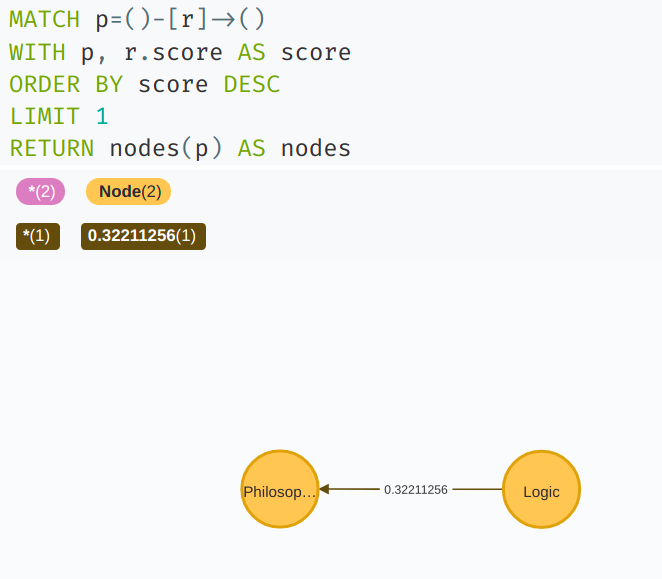
\includegraphics[width=200pt]{template/MaxNodes.png}
    \vspace*{-4mm}
    \caption{Pair of nodes with the highest similarity}
    \label{HighSim}
\end{figure}


\end{document}

%% NEWWWW CAREFUL

\documentclass[sigconf]{acmart}
\usepackage{algorithm} 
\usepackage{algpseudocode}

 
\algdef{SE}% flags used internally to indicate we're defining a new block statement
[STRUCT]% new block type, not to be confused with loops or if-statements
{Class}% "\Struct{name}" will indicate the start of the struct declaration
{EndClass}% "\EndStruct" ends the block indent
[1]% There is one argument, which is the name of the data structure
{\textbf{struct} \textsc{#1}}% typesetting of the start of a struct
{\textbf{end struct}}% typesetting the end of the struct


\begin{document}


\title{On building a transfer graph for the evolution of pages in Wikipedia}



\author{César Di Meglio, 2042789}
\affiliation{%
  \institution{Utrecht University}}
\email{c.t.dimeglio@students.uu.nl}




\maketitle

\section{Introduction}
The velocity aspect of Big data leads to evolution and change over time in the information considered. Keeping track of those changes contributes into a better understanding of how data behaves with respect context throughout time. In this project, we measure the similarity of pairs of Wikipedia pages. If we consider one Wikipedia page, measuring its similarity to other pages can be an indicator of a trend. For instance, if we consider the page "Big data", modifications are made to it over time. These modifications will increase or decrease its similarity to other pages. At one time step, "Big data" could be more similar to "Apache Spark" than "SQL". This would mean that "Apache Spark" plays a larger role in "Big data" than "SQL" at the given timestep. The main challenge is to match the timesteps of our data. That is to say, we need to compare pages that have existed together at the same point in time. Aggregating these comparisons may serve as a representative estimate of how two pages relate to one another given a time frame (section \ref{sim entities}).\\*
How can we measure the temporal similarity of pages in time ?
The latter will be problematized in section \ref{problem}, solutions will be presented in section \ref{solutions}.
\section{Problem Statement}
\label{problem}
\subsection{Wikipedia pages as entities}
We denote $W$ as a set of Wikipedia pages, referred to as "entities". Each entity $w \in W$ is updated over time by Wikipedia users, we call each of those updates \emph{versions}. 
For each entity, we only consider the \emph{references} to other Wikipedia pages with respect to its versions. For instance, the entity "Utrecht" will have hyperlinks pointing to other pages like "The Netherlands" or "Amsterdam" given one of its versions.\\
Some pages are more or less regularly updated, we denote $\mathcal{N}(w) \in \mathbb{N}^*$ as the total number of versions since the creation of entity $w$ on Wikipedia. More formally, we have the following:\\
Let $w_i$ be a version of $w$ at a timestep $i$.
\begin{equation}
    \label{references}
    \forall w \in W ,\; \forall i \in \{1,..\mathcal{N}(w)\}, \; w_i = \{r_1,r_2,..\}
\end{equation}
where $r_j$ are the \emph{references} (to other Wikipedia pages) present in $w_i$.
The \textbf{release \emph{date} of version} $w_i$ is noted $\tau(w_i)$.
There are no versions of $w$ that where released at the exact same date (Eq.\ref{chrono}), these chronologically ordered (Eq.\ref{ordered}).
\begin{equation}
    \label{chrono}
    \forall (i,j) \in \{1,..\mathcal{N}(w)\}^{2} \;| \; \tau(w_{i}) \neq \tau(w_{j})
\end{equation}
\begin{equation}
    \label{ordered}
    \tau(w_1) < \tau(w_2) < ... < \tau(w_{\mathcal{N}(w)})
\end{equation}
where the relation "$<$" here means that the version on the left was released prior to the version on the right. The version $w_{\mathcal{N}(w)}$ is the latest one, that is to say, the one being displayed when searching $w$ on Wikipedia. 
From one version to another, \emph{references} can either be added, removed or kept the same.\
Let $w_i$ and $w_j$ be two versions of $w$ such that $\tau(w_i)<\tau(w_j)$, $(i,j) \in  \{1,..\mathcal{N}(w)\}$\\*
Either one of these three cases can happen:
\begin{equation}
    \begin{cases}
    \label{scenarios}
    w_i = w_j & \text{no new references were added from $i$ to $j$} \\
    w_i \subseteq w_j & \text{new references were added from $i$ to $j$} \\
    w_i \not\subseteq w_j & \text{references were deleted from $i$ to $j$}
    \end{cases}
\end{equation}
Note that in the third case of (\ref{scenarios}): $w_i \not\subseteq w_j$, new references could also have been added into version $w_j$.
\subsection{Measuring the similarity of entities}
\subsubsection{Definition: Measuring similarity}:\\
\label{blackbox sim}
We denote $ \mu : W \times W \rightarrow [0,1]$ a function that computes the similarity of two Wikipedia distinct \footnote{We neglect cases were $w$=$w'$ as property (\ref{prop}) always holds} pages $w$ and $w'$. Let $\epsilon \in ]0,1[$ be the \emph{similarity threshold}. We define the following property:
\begin{equation}
    \label{prop}
    (w,w') \in W^{2}, \,\mu (w,w') \geq \epsilon \iff w \text{ and } w' \text{are similar}
\end{equation}

\subsubsection{Similarity metric for two versions}:\\
\label{sim versions}
The similarity metric chosen to compare two versions of two Wikipedia pages is the \emph{Jaccard similarity}:
\begin{equation}
    \label{compare versions}
    \mu (w_i,w'_{j}) = \frac{\sharp(w_i\cap w'_{j})}{\sharp(w_i\cup w'_{j})}
\end{equation}
It consists of the ratio of the cardinalities of the intersection and the union of $w_i$ and $w'_{j}$. The latter measures the similarity in between the sets $w_j$ and $w'_{j}$ which contain references to other Wikipedia pages. This is a commonly used metric for measuring set similarity. It is also \emph{commutative} i.e: $\mu (w_i,w'_{i}) = \mu (w'_{i},w_i)$. If we had chosen a metric without this property, then we would have needed to make twice as much comparisons. Moreover, it fulfills the properties of the function evoked to in section \ref{blackbox sim}.
\subsubsection{Similarity metric for two entities}:\\
\label{sim entities}
In the scope of this project, we want to compare two Wikipedia pages given their respective histories. For the latter, the versions of the entities are computed using the metric defined in \ref{sim versions}. We say that a version of an entity is \emph{displayed}, if it is the one that appears when the entity is searched on Wikipedia at a given point in time.
The challenge is that we must compare versions of entities that were \emph{displayed} at the same time. 
\begin{figure}[H]
    \centering
    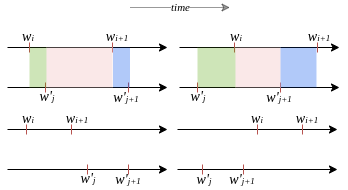
\includegraphics[width=200pt]{template/TimeDiff.png}
    \vspace*{-4mm}
    \caption{Overlapping configurations for $w_i$ and $w_j'$}
    \label{Overlap}
\end{figure}
Let $w$ and $w'$ be two entities we want to compare given their respective histories (see Fig. \ref{Overlap}). A version $w_i$ is \emph{displayed} from $\tau(w_i)$ included to $\tau(w_{i+1})$ excluded, $i \in \{1,...,\mathcal{N}(w)-1\}$.
In Fig.\ref{Overlap}, the two examples at the top (with the colors) exhibit configurations where versions can be compared because they are \emph{displayed} together at a point in time. Hence, for these examples, the following comparisons can be made :
\begin{equation}
    \begin{cases}
    \text{Top Left}: \mu(w_i,w'_j), \mu(w'_j,w_{i+1}), \mu(w_{i+1},w'_{j+1}) \\
    \text{Top Right}: \mu(w'_j,w_i), \mu(w_i,w'_{j+1}), \mu(w'_{j+1},w_{i+1})
    \end{cases}
\end{equation}
Those examples are non exhaustive. The gist main gist is that we must compare versions that we once up on Wikipedia at the same time.
In the case where $w_{i+2}$ and $w'_{j+2}$ are released before $w'_{j+1}$ and $w_{i+1}$ in the Top Left and Top right configurations respectively, the suited comparisons are made accordingly.
%$\mu(w_{i+2},w'_{j+1})$, $\mu(w'_{j+2},w_{i+1})$.

The two configurations (without colors) at the bottom illustrate the scenarios of time intervals where no comparison is possible since the versions are not \emph{displayed} at the same time. Let $\aleph$ (Bottom Left) and $\aleph'$ (Bottom Right) be the sets of pairs that describe these configurations:
\begin{equation}
    \begin{cases}
    \aleph = \{(w_i,w'_j)\;| \;(\tau(w_i)<\tau(w'_{j+1})) \land (\tau(w_{i+1})<\tau(w'_{j})) \}\\
    \aleph' = \{(w_i,w'_j)\;| \;(\tau(w_i)>\tau(w'_{j+1})) \land (\tau(w_{i+1})>\tau(w'_{j}))\}\\
    \textbf{with } (i,j) \in \{1,...,\mathcal{N}(w)-1\}\times\{1,...,\mathcal{N}(w')-1\}
    \end{cases}
\end{equation}
If we omit these cases for all timesteps, then we can retrieve all of the pairs $(w_i,w'_{j})$ of $w$ and $w'$ that were once \emph{displayed} at a same point in time. This set is noted $\Theta(w,w')$.
Hence, we want to compare such pairs of versions of $w$ and $w'$:
\begin{equation}
    \label{legal pairs}
    \Theta(w,w')= \{(w_i,w'_j)\:| \:(w_i,w'_j) \notin \aleph \cup \aleph'\}
\end{equation}
\textbf{with $(i,j) \in \{1,...,\mathcal{N}(w)\}\times\{1,...,\mathcal{N}(w')\}$}\\
Lastly, we need to aggregate the similarities of all of the "legal" comparisons to be made between the versions of $w$ and $w'$. For this, we take the mean of the similarities of each pairs of versions, noted $M(w,w')$. 
\begin{equation}
    \label{Mean}
    M(w,w') = \frac{1}{\sharp \Theta(w,w')}\sum_{(w_i,w'_j)\: \in \:\Theta(w,w')}\mu (w_i,w'_{j})
\end{equation}
Note that $M$ still fulfills the properties mentioned in section \ref{sim versions}, and especially the property \ref{prop} for two entities $w$ and $w'$. Our metric (Eq.\ref{compare versions}) can vary for two versions of a page. We then chose to take the mean (Eq.\ref{Mean}) to have a representative estimate of the similarity of pairs of entities throughout time.

\section{[Real]\:Dataset}
\label{realData}
In total, 30 entities were chosen arbitrarily. They all refer to either domains/sub-domains of Science (e.g Theoretical Physics, Topology..) or to famous scientists (e.g Marie Curie). For each \textbf{\texttt{entity}}, the following procedure was performed:\\*
- The links (to the previous versions) are fetched from the HTML code of the page:\\
https://en.wikipedia.org/w/index.php?title=\textbf{\texttt{entity}}\&action=history\\
using the API "Beautiful Soup".\\ 
The number of previous versions to be shown at once on this page can be set by tweaking the link above. We chose the maximum amount (approximately 5100). From one page to another, the number of previous existing versions can vary greatly with regard to how "famous" it is. For instance, Japanese DJ "Nujabes" only has a handful number of versions compared to the actor "Keanu Reeves". 
In this respect, we split the notoriety of the entities into three categories:
\begin{itemize}
    \item Low entities: pages with a history of less than 1000 versions
    \item Medium entities: pages with a history of 1000 to 5000 versions
    \item High entities: pages with a history of more than 5000 versions
\end{itemize}
The challenge is that for pages that are updated on a very regular basis (which are usually "High entities"), all of the versions available from the link above will span from now to at most three years (approximately) in the past. 
Whereas the versions from "Low entities" and "Medium entities" will span from now up to several years back in time (up to the very first version of the page).\\
For Low entities, we chose one version per year.
For Medium entities, we chose two versions per year.
For High entities, we chose 5 version per year.

- For each version that we select, the names of the references to other Wikipedia pages are collected (Eq.\ref{references}). As a result, for a single version, we obtain a vector of such a form:
\begin{equation}
    [date, r_1,r_2,...]
\end{equation}
The versions ("vectors") are then stored in separate files with respect to the entity they belong to. The advantage the way we generate our data is that we do not directly download the pages. We only retrieve the expected content which yields a lightweight dataset : 17.9 MB for the 30 entities. The latter could be interesting if we were to collect data from 100000 entities for example, this would ensure the dataset is as lightweight as possible.
\newpage
\section{Solution}
\label{solutions}

\subsection{Map-Reduce}
The Map Reduce solution Alg.\ref{MapRed} makes use of two procedures (functions) : \texttt{Map} and \texttt{Reduce}. The \texttt{Map} function, takes the dataset and maps "allowed" version pairs (Eq.\ref{legal pairs}), to a unique \texttt{Id} with respect to distinct pairs of entities. For these legal pairs, we check their pairs of versions that can be compared i.e: the ones belonging to their  $\Theta$ set (line 7). Each unique pair is attributed an unique key (line 8).
The latter distributes pair of versions to machines in order to parralellize the comparison computation.  Next, the \texttt{Reduce} function is in charge of computing the mean Jaccard similarity (Eq. \ref{Mean}) of two entities by regrouping the value pairs by their appropriate keys (\texttt{Id}s). A list of the pairs of versions at the previous step is taken as input, an iteration is performed over those pairs with respect to their ID (nested loops line 16 and 17). For each version the Jaccard similarity $\mu$ is computed. Once all of the Jaccard similarities of a unique pair are computed, the mean $\Mu$ is calculated (line 21). The function then outputs pairs of entities whose mean Jaccard similarity is at least $\epsilon$ (Eq.\ref{prop}) with their similarity (Eq.\ref{Mean}).


\begin{algorithm}
      \caption{Jaccard Map Reduce}
      \label{MapRed}
      \begin{algorithmic}[1]
        \Procedure{Map}{$D$}
        \State \Comment{Only \textbf{distinct} pairs of entities are considered because of the commutativity of our metric}
        \For{$(A,B) \in \{S \in \mathcal{P}(D)|\: \sharp S =2\}$} 
        \State \texttt{Id} $\gets$ Assign unique a unique key to every (A,B) pair 
        \For{$v \in$ \emph{list}(\{$v \in B$\})]} \Comment{Iterate over versions of $A$}
        \For{$v'\in$ \emph{list}(\{$v \in B$\})} \Comment{Iterate over versions of $B$}
        \If{$(v,v') \in \Theta(A,B)$} 
        \State \texttt{Emit}(\texttt{Id}, pair($v,v'$)) 
        \EndIf
        \EndFor
        \EndFor
        \EndFor
        \EndProcedure
        
        \Procedure{Reduce}{\texttt{Id}, pairs: [$p_1,p_2..,$] ,$\epsilon$} 
        \State Sum $\gets 0$
        \For{\texttt{Id} in $list$(\texttt{Id})} \Comment{$list$(\texttt{Id}): list of the keys \texttt{Map} created}
        \For{$p \in P_{\texttt{Id}}$} \Comment{$P_{\texttt{Id}}$: set of pairs of with the same \texttt{Id}}
        \State Jaccard = $\mu(p)$ \Comment{(Eq.\ref{compare versions})}
        \State Sum $\gets$ Sum + Jaccard
        \EndFor
        \State M $\gets \frac{1}{\sharp P_{\texttt{Id}}}\cdot$Sum
        \If{M$\geq \epsilon$}
        \State \texttt{Emit}(\texttt{Id}, M)
        \EndIf
        \EndFor
        \Comment{(Eq.\ref{Mean})}
        \EndProcedure
    \end{algorithmic}
\end{algorithm}

\newpage
\subsection{Spark}
The Spark solution Alg.\ref{Spark} accepts the data $D$ and a threshold $\epsilon$. After empirical analysis, we chose $\epsilon=0.015$ as the threshold (Prop.\ref{prop}). This rather low value was intentionally chosen to be able to show as much relevant relationships as possible. Generally, entities that can intuitively be considered as similar  like "Database" and "Big data" have a relatively low Jaccard similarity (under $0.4$ from empirical testing).\\*
We start by defining an empty \texttt{spark.DataFrame}: $Result$. This dataframe has three columns (or "headers"): EntityA, EntityB and "Jaccard similarity". Here as well, only distinct pairs (EntityA, EntityB) of entities are considered. For every of those pairs we compute $\Theta(A,B)$, the versions which we are "allowed" to compare from EntityA and EntityB (Eq.\ref{legal pairs}). The computation of such a set is done using Resilient Distributed Datasets (RDDs), hence the $\texttt{RDD}\langle .\rangle$ operator at line 6. This set is then converted into a \texttt{spark.DataFrame}: $DF$ with headers : EntityA and EntityB. For each of the version pairs of those entities (i.e for each row, line 7), the Jaccard similarity (Eq.\ref{compare versions}) of EntityA and EntityB is computed and stored in a new column for $DF$ : "Jaccard" (line 8). The mean (Eq.\ref{Mean}) Jaccard similarity of those entities is then computed. If it is a least greater than the desired threshold $\epsilon = 0.015$ (Prop.\ref{prop}), then a row is concatenated to $Result$ by matching its schema, names of entity A and B, as well as their Jaccard similarity.


\begin{algorithm}
  \begin{algorithmic}[1]
    \caption{Jaccard Spark}
    \label{Spark}
        \Procedure{Jaccard Calculator}{$D$,$\epsilon$}
        \State $P$ \gets $\{S \in \mathcal{P}(D)|\: \sharp S =2\}$
        \Comment{Set of pairs from dataset $D$}
        \State $Result$ $\gets \texttt{spark.DataFrame}(\emptyset)$ \Comment{Empty Dataframe}
        \For{$(A,B) \in P $}
        \State $\Theta \gets \texttt{RDD}\langle\Theta (A,B)\rangle$
        \State $DF \gets \texttt{spark.DataFrame}(\Theta)$
        \For{row in $DF$} \Comment{headers: [EntityA,EntityB]}
        \State $DF\text{[Jaccard]} \gets \mu (DF[\text{EntityA}],DF[\text{EntityB}])$
        \EndFor
        \State M$\gets M(DF[\text{Jaccard}])$ \Comment{Mean of Jaccard column}
        \If{M $\geq \epsilon$}
        \State $Result = Result \:||\:\text{Row}(A,B,M)$
        \EndIf
        \State \textbf{return} $Result$
        \EndProcedure
  \end{algorithmic}
\end{algorithm}

\section{Loading}
\subsection{Loading}
The resulting data from Alg.\ref{Spark} was loaded into Neo4J Desktop. First, an index named "Node" was created on the names of the entities. The nodes were loaded into Neo4j with the \texttt{Nodes.csv} file were the index was applied for every entity. The relationships were then loaded with the \texttt{Links.csv} file. We then queried Neo4j to match the nodes that have a link and to show the value of their Jaccard similarity on the edges. This was realized using the "APOC" plugin for Neo4j databases. Please note that no attention needs to be payed at the direction of the edges since our metric is commutative. Moreover, Neo4j does not support undirected edges.
\subsection{Nodes with the highest similarity}
The following Cypher query was used to find the pair of entities with the highest similarity:\\*
1. \texttt{MATCH p=()-[r]->()}\\*
2. \texttt{WITH p, r.score AS score}\\*
3. \texttt{ORDER BY score DESC}\\*
4. \texttt{LIMIT 1}\\*
5. \texttt{RETURN nodes(p) AS nodes}\\*
We first select the relations and their value (lines 1 and 2), then order them in decreasing order (line 3). Next, we limit the number of relationships values to be shown to one (line 4). The corresponding nodes to this relationship are returned (line 5). We obtain the output shown in Fig.\ref{HighSim}
\begin{figure}[H]
    \centering
    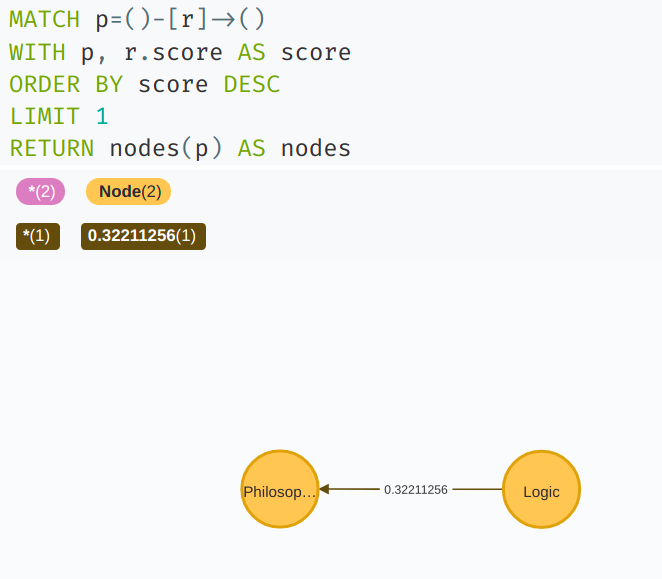
\includegraphics[width=200pt]{template/MaxNodes.png}
    \vspace*{-4mm}
    \caption{Pair of nodes with the highest similarity}
    \label{HighSim}
\end{figure}
%\newpage
\section{Experiments}
In order to demonstrate how our solution works, experiments were performed by looking how it scales with a given number of entities. A total of 120 entities were downloaded randomly from Wikipedia using the same technique as mentioned in \ref{realData}. We studied the time it took for the program to compute the solution with respect to the number of entities.
\\
Due to the sparsity of the references to other entities across versions, a threshold of $0.000005$ was chosen. Even if it seems quite low, two entities whose mean Jaccard similiraty Eq.\ref{Mean} is above it can safely be considered similar in terms of content.
Let $f: \mathbb{N}^{*} \rightarrow \mathbb{N}^{*}$ describe the number of comparisons to be made as a function of the number of entities considered. We then have:
\begin{equation}
    f(N) = {N\choose 2} =\frac{N!}{2!(N-2)!} = \frac{N(N-1)}{2}
\end{equation}
    The main drawback to our program, is that regardless of the threshold we select, we still have to compute the Jaccard similarity to ensure two entities are below the given threshold. Note that for each pair of entities $(A,B)$, we have to compare $\sharp \Theta (A,B)$ versions. In order to speed up the process, \textbf{the code to Alg.\ref{Spark} was slightly changed}: if the intersection of two versions is the empty set, then it skips the computation and does not bother calculating the Jaccard similarity.
\begin{figure}[H]
    \centering
    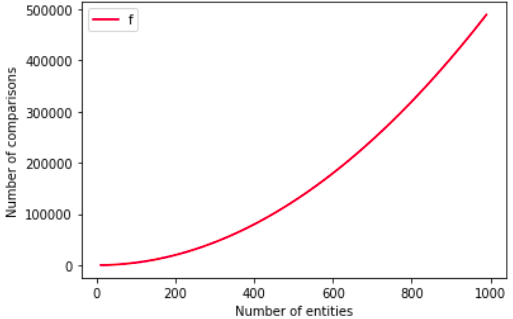
\includegraphics[width=200pt]{template/NchooseK.png}
    \vspace*{-4mm}
    \caption{Comparisons as a function of the entities}
    \label{factorial}
\end{figure}
The following plot aims to exhibit the complexity of our program with respect to the number of entities. The number of entities considered (from 10 to 120) is not high enough to truly infer the behaviour of the complexity curve. The program was ran on one machine (Intel(R) Core(TM) i7-8750H CPU @ 2.20GHz). It would be more scalable by using a more powerful CPU or running it across a cluster of machines, hence the time complexity could be further diminished. Moreover, the contribution to time complexity does not come from the size of the data since we collect it in an effective and lightweight manner Section.\ref{realData}. It comes from the sheer amount of one-to-one comparisons to be made.
Fig.\ref{complexity}
\begin{figure}[H]
    \centering
    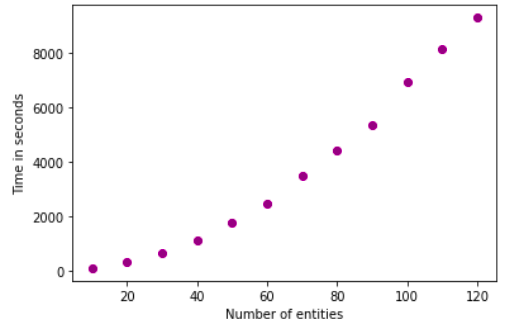
\includegraphics[width=200pt]{template/CompSOL.png}
    \vspace*{-4mm}
    \caption{Time complexity of Alg.\ref{Spark}}
    \label{complexity}
\end{figure}
From this concave plot, we can make the hypothesis that our program has a polynomial time complexity. To further support our hypothesis, we took the natural logarithm of Fig.\ref{complexity}, we obtain a non-linear convex curve Fig.\ref{Lcomplexity} which argues it is not exponential.
\vspace*{-2mm}
\begin{figure}[H]
    \centering
    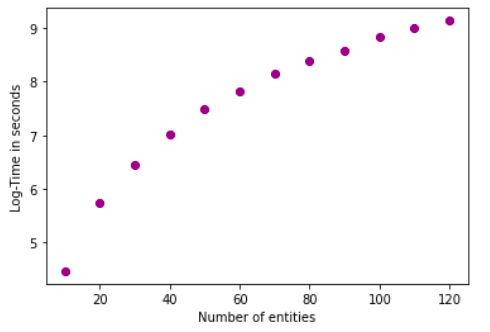
\includegraphics[width=200pt]{template/LOGtime.png}
    \vspace*{-4mm}
    \caption{Log-Time complexity of Alg.\ref{Spark}}
    \label{Lcomplexity}
\end{figure}


\end{document}
















